v5.\+0.\+144 is a free software distributed under the \href{http://www.gnu.org/licenses/}{\tt G\+NU General Public License}.

(Q\+GD) is an optimization method to decompose an arbitrary NxN Unitary matrix into a sequence of \hyperlink{class_u3}{U3} and \hyperlink{class_c_n_o_t}{C\+N\+OT} gates. It is written in C/\+C++ providing a simple Python interface via \href{https://docs.python.org/3/library/ctypes.html}{\tt ctypes} and a possibility to run Q\+GD as a standalone C executable. The present package is supplied with automake tools to ease its deployment. The Q\+GD package can be built with both Intel and G\+NU compilers, and link against various C\+B\+L\+AS libraries installed on the system. (So far the C\+L\+B\+AS libraries of the G\+NU Scientific Library and the Intel M\+KL packages were tested.) In the following we briefly summarize the steps to build, install and use the Q\+GD package.

 
\begin{DoxyImageNoCaption}
  \mbox{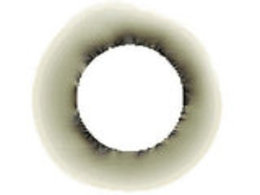
\includegraphics[width=\textwidth,height=\textheight/2,keepaspectratio=true]{intro_wavefunc.jpg}}
\end{DoxyImageNoCaption}


The project was supported ... H\+U\+N\+QT ...

\section*{Dependencies}

The optimization algorithm of Q\+GD relies on the \href{https://www.gnu.org/software/gsl/doc/html/multimin.html}{\tt multimin} component of the \href{https://www.gnu.org/software/gsl/doc/html/index.html}{\tt G\+NU Scientific Library}. We developed and tested the Q\+GD package with G\+NU Scientific Library of version 2.\+5 and 2.\+6. The dependencies necessary to compile and build the Q\+GD package are the followings\+:


\begin{DoxyItemize}
\item \href{https://www.gnu.org/software/automake/}{\tt automake} (for further development purposes)
\item \href{https://www.gnu.org/software/autoconf/}{\tt autoconf} (for further development purposes)
\item \href{https://www.gnu.org/software/libtool/}{\tt libtool}
\item \href{https://www.gnu.org/software/make/}{\tt make}
\item \href{https://www.gnu.org/software/gsl/doc/html/index.html}{\tt G\+NU Scientific Library} ($>$=2.\+5)
\item C++/C \href{https://software.intel.com/content/www/us/en/develop/tools/compilers/c-compilers.html}{\tt Intel} or \href{https://gcc.gnu.org/}{\tt G\+NU} compiler
\item \href{https://software.intel.com/content/www/us/en/develop/tools/math-kernel-library.html}{\tt Intel M\+KL} (optional)
\end{DoxyItemize}

The Python interface of Q\+GD was developed and tested with Python 3.\+6 and 3.\+7. The Q\+GD Python interface needs the following packages to be installed on the system\+:


\begin{DoxyItemize}
\item \href{https://qiskit.org/documentation/install.html}{\tt Qiskit}
\item \href{https://numpy.org/install/}{\tt Numpy}
\item \href{https://www.scipy.org/install.html}{\tt scipy}
\item \href{https://docs.python.org/3/library/ctypes.html}{\tt ctypes}
\end{DoxyItemize}

\section*{How to build G\+NU Scientific Library}

If the G\+NU Scientific Library is not installed on the system, it can be easily compiled and deployed by the end user without administrative privileges. The G\+NU Scientific Library can be downloaded from the site \href{https://www.gnu.org/software/gsl/}{\tt https\+://www.\+gnu.\+org/software/gsl/}. After the downloaded package is extracted somewhere in the home directory of the user ({\bfseries path/to/gslsource}), one should configure the compiling environment using the {\bfseries configure} tool. Depending on the individual settings the default compiler to be invoked might be different from H\+PC to H\+PC. To ensure the usage of the G\+NU compiler, the following shell command should be executed inside the directory {\bfseries path/to/gslsource}\+:

\$ ./configure --prefix=path/to/gsl FC=gfortran CC=gcc C\+XX=g++

(Similarly, Intel compiler can be forced by setting FC=ifort CC=icc and C\+XX=icpc.) The installation directory of the compiled G\+NU Scientific Library is given by --prefix=path/to/gsl (which is different from the directory path of the source files given by {\bfseries path/to/gslsource}). To install G\+NU Scientific Library the user should have read and write permissions on the path {\bfseries path/to/gsl} (which might be for example /home/username/gsl). After the successful configuration the G\+NU Scientific Library can be compiled by the shell command

\$ make

The compilation of the G\+NU Scientific Library takes some time. When the compilation is done, the package (including the C header files and the static and shared libraries) is installed into the directory {\bfseries path/to/gsl} by the shell command\+:

\$ make install

\section*{Download the Quantum Gate Decomposer package}

The developer version Quantum Gate Decomposer package can be downloaded from github repository \href{https://github.com/rakytap/quantum-gate-decomposer/tree/C++}{\tt https\+://github.\+com/rakytap/quantum-\/gate-\/decomposer/tree/\+C++}. After the downloaded package is extracted into the directory {\bfseries path/to/qgdsource} (which would be the path to the source code of the Q\+GD package), one can proceed to the compilation steps described in the next section.

\section*{How to deploy the Quantum Gate Decomposer package}

Similarly to G\+NU Scientific Library, the Q\+GD package is also equipped with automake tools to ease the compilation and the deployment of the package. To ensure that Q\+GD package would find the necessary libraries and header files during compilation time it is advised to define the following environment variables\+:

\$ export G\+S\+L\+\_\+\+L\+I\+B\+\_\+\+D\+IR=path/to/gsl/lib(64)

\$ export G\+S\+L\+\_\+\+I\+N\+C\+\_\+\+D\+IR=path/to/gsl/include

When using Intel compiler equipped with Intel M\+KL on a H\+PC, the compiler can find his way to the M\+KL libraries automatically through the environment variable M\+K\+L\+R\+O\+OT which points to the root directory of the M\+KL package. If the Intel environment variables are not set, they can be initialized by the shell command\+:

\$ source /opt/intel/composerxe/bin/compilervars.sh intel64

where /opt/intel/composerxe is the path to the Intel compiler package location which might be different from the given one. (This step can be omitted when using G\+NU compiler, or when we do not have intention to use Intel M\+KL) After the basic environment variables are set, the compilation can be configured by the command executed in the source directory {\bfseries path/to/qgdsource} of the Q\+GD package\+:

\$ ./configure --prefix=path/to/qgd CC=gcc C\+XX=g++

where path/to/qgd is the installation path of the Quantum Gate Decomposer package. The installation directory of the compiled Q\+GD package is given by --prefix=path/to/qgd (which is different from the directory path of the source files given by {\bfseries path/to/qgdsource}). The user should have read and write permissions on the path {\bfseries path/to/qgd} (which can be for example /home/username/qgd). Another optional flag --enable-\/ffast-\/math enables the compiler\textquotesingle{}s floating-\/point optimization (which is usually enabled by default in Intel compilers settings). While in general this optimization is considered to be dangerous, the runtime performance might be significantly increased due to this optimization. Try to compile without and with this flag and compare the performance and stability of the resulted binaries (for further information see section {\bfseries How to use}). We notice, that the Q\+GD Python interface does not fully support this optimization resulting in lower performance than a standalone C applications. On the other hand, if one choses Intel compiler to built the Q\+GD package, the following configuration settings should be invoked\+:

\$ ./configure --prefix=path/to/qgd --with-\/mkl CC=icc C\+XX=icpc

The --with-\/mkl flag sets the appropriate linking of the Q\+GD package with the Intel M\+KL package. If the flag is missing from the configuration than the C\+B\+L\+AS library of the G\+NU Scientific Library is used for linear algebra operations. After the successful configuration the Q\+GD package can be compiled by the shell command executed in the directory {\bfseries path/to/qgdsource}\+:

\$ make

After a successful compilation of the Q\+GD package, it can be installed into the directory {\bfseries path/to/gsl} by the shell command\+:

\$ make install

The installation procedure will copy all the C header files, the static and shared libraries needed for further developments and the python interface files including a simple python example file {\bfseries \hyperlink{example_8py}{example.\+py}} into the installation destination defined by the {\bfseries path/to$\ast$qgd} path.

\section*{How to use}

The algorithm implemented in the Q\+GD package intends to transform the given unitary into an identity matrix via a sequence of \hyperlink{class_c_n_o_t}{C\+N\+OT} and \hyperlink{class_u3}{U3} operations applied on the unitary. Thus, in order to really get the decomposition of a unitary, one should rather provide the complex transpose of this unitary as the input for the Q\+GD decomposing process.

\subsection*{Standalone executable}

During the compilation and the installation processes of the Q\+GD package a standalone executable was also built and copied into the directory {\bfseries path/to/gsl/bin}. This executable can be executed by a command

\$ ./decomposition\+\_\+test

and it starts a decomposition of a random general unitary matrix. The source of this example is located in {\bfseries path/to/qgdsource/test\+\_\+standalone/} and shows a simple test case of the usage of the Q\+GD package. The Doxygen documentation of the Q\+GD A\+PI can be also generated in order fully exploit the functionalities of the Q\+GD package (for further details see section {\bfseries Doxygen manual} at the end of this manual).

\subsection*{Python Interface}

The Q\+GD package contains a simple python interface allowing the access of the functionalities of the Q\+GD package from Python. The usage of the Q\+GD Python interface is demonstrated in the example file {\bfseries \hyperlink{example_8py}{example.\+py}} located in the directory {\bfseries path/to/qgd} and can be run similarly to any python scripts. The example file imports the {\bfseries \hyperlink{namespaceqgd__python}{qgd\+\_\+python}} module containing the wrapper class for the decomposition of a given unitary matrix. The wrapper class loads the shared library libqgd.\+so and performs the data conversion between the python and C sides.

It should be noted, however, that the python interface functions are implemented only for few functionalities of the whole Q\+GD A\+PI. Another desired interface functions can be implemented following the source of already implemented interface function in source file {\bfseries \hyperlink{python__interface_8cpp}{python\+\_\+interface.\+cpp}} in the main directory of the Q\+GD source code.

\section*{development Development}

The Q\+GD A\+PI enables the extension of the capabilities of the Q\+GD packages into further projects. The Q\+GD header files needed for the compilation of the project are provided in the directory {\bfseries path/to/qgd/include}. The compiled object files should than be linked against the static or shared Q\+GD libraries libqgd.\+a or libqgd.\+so, respectively, located in the directory {\bfseries path/to/qgd/lib(64)}. In order to exploit the speedup comming from the floating point optimization, we notice that Intel\textquotesingle{}s compiler (usually) use this optimization by default, but when linking with G\+NU compiler, the -\/ffast-\/math option must be append when linking against the Q\+GD A\+PI library is done. The full documentation of the Q\+GD A\+PI can be accessed by a Doxygen manual which can be accessed and recreated by steps described in the following section 